%\documentclass[a4paper]{article}

%\documentclass[9pt,twocolumn,twoside, lineno]{gsajnl}
\documentclass[12pt,twoside, lineno]{gsajnl}
% Use the documentclass option 'lineno' to view line numbers
\usepackage{tabularx}
\usepackage{longtable}
\articletype{mp} % article type
% {inv} Investigation 
% {gs} Genomic Selection
% {goi} Genetics of Immunity 
% {gos} Genetics of Sex 
% {mp} Multiparental Populations

\title{Testing pleiotropy vs. separate QTL in multiparental populations}

\author[$\ast$,1]{Frederick J. Boehm}
\author[$\ast$, $\dagger$]{Brian S. Yandell}
\author[$\ddagger$]{Karl W. Broman}
\author[$\S$]{Author Four}
\author[$\ast\ast$]{Author Five}

\affil[$\ast$]{Department of Statistics, University of Wisconsin-Madison, Madison, Wisconsin 53706}
\affil[$\dagger$]{Department of Horticulture, University of Wisconsin-Madison, Madison, Wisconsin 53706}
\affil[$\ddagger$]{Department of Biostatistics and Medical Informatics, University of Wisconsin-Madison, Madison, Wisconsin 53706}
\affil[$\S$]{Author four affiliation}
\affil[$\ast\ast$]{Author five affiliation}

\keywords{Quantitative trait locus; pleiotropy; multivariate analysis; linear mixed effects models; systems genetics; ...}

\runningtitle{Testing pleiotropy vs. separate QTL} % For use in the footer 

%% For the footnote.
%% Give the last name of the first author if only one author;
% \runningauthor{FirstAuthorLastname}
%% last names of both authors if there are two authors;
% \runningauthor{FirstAuthorLastname and SecondAuthorLastname}
%% last name of the first author followed by et al, if more than two authors.
\runningauthor{Boehm \textit{et al.}}




\begin{abstract}
%The abstract should be written for people who may not read the entire paper, so it must stand on its own. The impression it makes usually determines whether the reader will go on to read the article, so the abstract must be engaging, clear, and concise. In addition, the abstract may be the only part of the article that is indexed in databases, so it must accurately reflect the content of the article. A well-written abstract is the  most effective way to reach intended readers, leading to more robust search, retrieval, and usage of the article. 
Simultaneous developments of model organism multiparental populations with high mapping resolution and of technologies to measure tens of thousands of phenotypes present an opportunity for quantitative methods to enhance understanding of complex trait architecture. In multivariate quantitative trait locus mapping studies, one often observes multiple traits that map to a single genomic region. In this setting, knowing the number of distinct loci informs understanding of complex trait architecture and planning for subsequent experiments. We extend the work of \citet{jiang1995multiple} to develop a likelihood ratio test for the alternative hypothesis of separate QTL of two loci against the null hypothesis of pleiotropy for a pair of traits that map to a single genomic region. Unlike previous tests of these competing hypotheses, our test incorporates polygenic random effects to account for complex patterns of relatedness among subjects. Additionally, our test accommodates more than two founder alleles. We use a parametric bootstrap to determine statistical significance. Finally, we apply our methods to a behavioral genetics data set from Diversity Outbred mice, where we find evidence for presence of two distinct loci in a 2.5-centiMorgan region on Chromosome 8, where one locus affects "percent time in light" and a second, distinct locus affects "hot plate latency". We share our software in an accessory R package, \texttt{qtl2pleio} on Github.

%Please see additional guidelines notes on preparing your abstract below.
\end{abstract}
%%%%%%%%%%%%%%%%%%%%%%%%%%%%%%%%%%%%%%%%%%
% Stuff between the two lines of percentage marks may need to be removed before the draft is finalized.
\usepackage[colorinlistoftodos, prependcaption,textsize=tiny]{todonotes}
%% use 'disable' option for todonotes to disable the package, as in the commented line below. 
% \usepackage[disable, colorinlistoftodos, prependcaption,textsize=tiny]{todonotes}
\presetkeys%
    {todonotes}%
    {inline,backgroundcolor=yellow}{}

%%%%%%%%%%%%%%%%%%%%%%%%%%%%%%%%%%%%%%%%%%
\setboolean{displaycopyright}{true}

\begin{document}

\maketitle
\thispagestyle{firststyle}
\marginmark
\firstpagefootnote
\correspondingauthoraffiliation{Department of Statistics, 1220 Medical Sciences Center, 1300 University Avenue, Madison, WI 53706. E-mail: frederick.boehm@gmail.com} %Please insert the affiliation correspondence address and email for the corresponding author. The corresponding author should be marked with a `1' in the author list, as shown in the example.}
\vspace{-11pt}%

%\lettrine[lines=2]{\color{color2}T}{}his \textit{Genetics} journal template is provided to help you write your work in the correct journal format. Instructions for use are provided below. 




% try to zoom from big picture to my specific questions



Complex trait studies in multiparental populations present new challenges in statistical methods and data analysis. Among these is the development of strategies for multivariate trait analysis. While examining one trait at a time has become standard practice in mapping quantitative trait loci (QTL), we argue below that simultaneous analysis of two or more traits in multiparental populations addresses additional questions, including the ability to ask whether two traits share a single pleiotropic locus. We present below a statistical hypothesis test to address this question. We characterize our test's statistical properties and apply it to publicly available data from Diversity Outbred mice to learn that two behavioral traits that map to a 2.5-cM region arise from two separate QTL.


%In a 2014 systems genetics study of behavioral traits, \citet{recla2014precise} identified a gene on chromosome 8, \textit{Hydin} (axonemal central pair apparatus protein; MGI:2389007), that associates with thermal pain response in Diversity Outbred (DO) mice \citep{churchill2012diversity, svenson2012high}. While a molecular mechanism for this relationship remains unclear, \citet{recla2014precise} reasoned that \textit{Hydin}'s gene product, a protein, might impact ciliary motility in cerebral spinal fluid of the brain.

%In our analyses of 26 phenotypes from \citet{recla2014precise} and its companion report \citep{logan2013high}, we identified two additional traits that, when considered individually, map to the same region of chromosome 8 as does thermal pain response. \citet{logan2013high} originally reported these associations, but didn't reach conclusions about the underlying genes. This prompted us to ask the question ``Are there multiple underlying loci, or is there a single pleiotropic locus'' for these three traits, thermal pain response, percent time in light, and distance traveled in light. 


Previous research addressed the question of pleiotropy vs. separate QTL in two-parent crosses. To gain insight into genetic architecture of complex traits, \citet{jiang1995multiple} developed a likelihood ratio test for pleiotropy vs. separate QTL. For two traits that map to a single genomic region, they fit null models in which a single QTL affects two traits and alternative models in which two distinct QTL affect one trait each.  \citet{jiang1995multiple} argued that distinguishing between these two hypotheses - pleiotropy and separate QTL - informs understanding of genetic architecture of complex traits. \citet{knott2000multitrait} used linear regression to develop a fast approximation to the test of \citet{jiang1995multiple}, while \citet{tian2016dissection} used the methods from \citet{knott2000multitrait} to dissect QTL hotspots in a F$_2$ population. In analyzing genome-wide expression traits, \citet{tian2016dissection} found evidence for the presence of at least two QTL in five of six expression trait hotspots.


Newly developed, community-supported multiparental populations, such as the Diversity Outbred mouse population, have enabled high-precision mapping of complex traits \citep{de2014genetics}. The Diversity Outbred mouse population began with progenitors of the Collaborative Cross mice \citep{churchill2004collaborative,churchill2012diversity}. Each Diversity Outbred mouse is a highly heterozygous genetic mosaic of alleles from the eight Collaborative Cross founder lines. Random matings among non-siblings have maintained the Diversity Outbred population for more than 23 generations \citep{chesler2016diversity}. 


Several limitations of previous pleiotropy vs. separate QTL tests prevent their direct application in multiparental populations. First, multiparental populations have complex patterns of relatedness among subjects, and failure to account for these patterns of relatedness may lead to spurious results \citep{yang2014advantages}. Second, previous tests allowed for only two founder lines \citep{jiang1995multiple}. Finally, \citet{jiang1995multiple} assumed that the null distribution of the test statistic follows a chi-square distribution.  

We developed a pleiotropy vs. separate QTL test for two traits in multiparental populations. Our test builds on research that \citet{jiang1995multiple}, \citet{knott2000multitrait}, \citet{tian2016dissection}, and \citet{zhou2014efficient} initiated. Our innovations include the accommodation of $k$ founder alleles per locus (compared to the traditional two founder alleles per locus) and the incorporation of multivariate polygenic random effects to account for relatedness. Furthermore, we implemented a parametric bootstrap to calibrate test statistic values \citep{efron1979,tian2016dissection}. 

Below, we describe our likelihood ratio test for pleiotropy vs. separate QTL. In simulation studies, we find that it is slightly conservative, and that it has power to detect two separate loci when the univariate LOD peaks are strong. We then apply our test to two behavioral phenotypes. We find modest evidence for two distinct QTL in a region on Chromosome 8 \citep{logan2013high,recla2014precise}. 


%For the introduction, authors should be mindful of the broad readership of the journal. The introduction should set the stage for the importance of the work to a generalist reader and draw the reader in to the specific study. The scope and impact of the work should be clearly stated.

%In individual organisms where a mutant is being studied, the rationale for the study of that mutant must be clear to a geneticist not studying that particular organism. Similarly, study of particular phenotypes should be justified broadly and not on the basis of interest for that organism alone. General background on the importance of the genetic pathway and/or phenotype should be provided in a single, well-reasoned paragraph near the beginning of the introduction.

%Authors are encouraged to:

%\begin{itemize}
%\item cite the supporting literature completely rather than select a subset of citations;
%\item provide important background citations, including relevant review papers (to help orient the non-specialist reader);
%\item to cite similar work in other organisms.
%\end{itemize}

\section{Methods}
\label{sec:materials:methods}

%Manuscripts submitted to \textit{GENETICS} should contain a clear description of the experimental design in sufficient detail so that the experimental analysis could be repeated by another scientist. If the level of detail necessary to explain the protocol goes beyond two paragraphs, give a short description in the main body of the paper and prepare a detailed description for supporting information.  For example, details would include indicating how many individuals were used, and if applicable how individuals or groups were combined for analysis. If working with mutants indicate how many independent mutants were isolated. If working with populations indicate how samples were collected and whether they were random with respect to the target population.

Our strategy involves first identifying two traits that map to one genomic region. We then perform a two-dimensional QTL scan over the genomic region. We identify the marker that maximizes the likelihood under pleiotropy and the ordered pair of markers that maximizes the likelihood under the two separate QTL model. The logarithm of the ratio of the two likelihoods is our test statistic. We then calibrate our test statistic with a parametric bootstrap. 

\subsection{Data structures}

We arrange the data into three objects. The first is a $n$ by $k$ by $m$ array of allele probabilities for n subjects with $k$ alleles per marker and $m$ markers on a single chromosome. The second object is a $n$ by $d$ matrix of phenotype values, where $d = 2$ for our analyses. Each column is a single phenotype and each row is a single subject. The third object is a $n$ by $c$ matrix of covariates, where each row is one subject and each column is one covariate. In analyses below, we use four indicator variables to specify each subject's sex and membership in one of four waves of subjects.

One additional object is the genotype-derived collection of ``leave one chromosome out'' kinship matrices. The ``leave one chromosome out'' approach calculates a collection of kinship matrices, one for each chromosome. Each kinship matrix results from kinship estimation performed while omitting the genetic data from a single chromosome. For example, the chromosome 1 ``leave one chromosome out'' kinship matrix results from omitting the genetic data of chromosome 1 and using all other genetic data. Our motivation for using ``leave one chromosome out'' kinship calculations is to avoid using any marker's genetic data in both the kinship matrix and a design matrix for linear mixed effects models \citep{yang2014advantages}. 


%\subsection{Allele probabilities inference}


%\citet{broman2012genotype,broman2012haplotype} developed hidden Markov model methods for genotype probability inference in recombinant inbred lines. We applied these methods, as implemented in the R package \texttt{qtl2}, to infer probabilities for each of the 36 states (8 homozygote and 28 heterozygote) at each marker. With the 36 genotype probabilities per mouse per marker, we calculated 8 founder allele probabilities per mouse per marker. 

\subsection{Statistical Models} 
The next step in a pleiotropy vs. separate QTL test, after identifying two traits and a genomic region of interest, is a two-dimensional QTL scan \citep{jiang1995multiple}. in a two-dimensional QTL scan, we fit the multivariate linear mixed effects model defined in Equation \ref{eqn:model1} once for every ordered pair of markers. Note that we assumed an additive genetic model throughout our analyses, but extensions to design matrices for dominance models are straightforward.


\begin{equation}
vec(Y) = X vec(B) + vec(G) + vec(E)
\label{eqn:model1}
\end{equation}
where $Y$ is a $n$ by $2$ matrix of phenotypes values, where each row is one mouse and each column is one trait; $X$ is a $2n$ by $2(k + c)$ matrix that contains two markers' $k$ allele probabilities and $c$ covariates in diagonal blocks; $B$ is a $(k + c)$ by $2$ matrix of allele effects and covariate effects; $G$ is a $n$ by $2$ matrix of random effects; and $E$ is a $n$ by $2$ matrix of random errors. $n$ is the number of mice. The `vec' operator stacks columns from a matrix into a single vector. For example, a 2 by 2 matrix inputted to `vec' results in a vector with length 4. Its first two entries are the matrix's first column, while the third and fourth entries are the matrix's second column.


We also impose distributional assumptions on $G$ and $E$:

\begin{equation}
G \sim MN_{n x 2}(0, K, V_g)
\label{eqn:model2}
\end{equation}

and

\begin{equation}
E \sim MN_{nx2}(0, I, V_e)
\label{eqn:model3}
\end{equation}
where $MN_{n x 2}(0, V_r, V_c)$ denotes the matrix-variate (n by 2) normal distribution with mean being the $n$ by $2$ matrix with all zero entries and row covariance $V_r$ and column covariance $V_c$. We assume that $G$ and $E$ are independent. 


\subsection{Parameter inference and log likelihood calculation}

Inference for parameters in multivariate linear mixed effects models is notoriously difficult and computationally intense \citep{meyer1989restricted,meyer1991estimating}. Thus, we make the simplifying assumption that $V_g$ and $V_e$ don't depend on allele probabilities. We use restricted maximum likelihood methods to fit the model:

\begin{equation}
vec(Y) = X_0vec(B) + vec(G) + vec(E)
\label{model}
\end{equation}
$X_0$ is a $2n$ by $2(c + 1)$ matrix. The first column of each diagonal block $X_0$ has all entries equal to one, and the remaining columns are covariates. 

We draw on our implementation \citep{gemma2} (in \texttt{R}) of the GEMMA algorithm for fitting a multivariate linear mixed effects model with expectation-maximization \citep{zhou2014efficient}. We use restricted maximum likelihood fits for the variance components $V_g$ and $V_e$ in subsequent calculations of the generalized least squares solution $\hat B$. 

\begin{equation}
    \hat B = (X^T\hat\Sigma^{-1}X)^{-1}X^T\hat\Sigma^{-1}vec(Y)
\end{equation}

\noindent where 

\begin{equation}
    \hat\Sigma = \hat V_g \otimes K + \hat V_e \otimes I_n
    \label{cov}
\end{equation}

\noindent where $\otimes$ denotes the Kronecker product, $K$ is a ("leave one chromosome out") kinship matrix, and $I_n$ is a n by n identity matrix. We then calculate the log likelihood for a normal distribution with mean $X vec(\hat B)$ and covariance $\hat \Sigma$ that depends on our estimates of $V_g$ and $V_e$ (Equation \ref{cov}). 

\subsection{Pleiotropy vs. separate QTL hypothesis testing framework}

Our test applies to two traits considered simultaneously. Below, $\omega_1$ and $\omega_2$ denote putative locus positions for traits one and two. We quantitatively state the competing hypotheses for our test as:

\begin{eqnarray}
H_0: \omega_1 = \omega_2 \nonumber\\
H_A: \omega_1 \neq \omega_2
\label{eqn:hypotheses}
\end{eqnarray}

\noindent Our likelihood ratio test statistic is:

\begin{equation}
- \log_{10} \frac{\max L_0(B, \Sigma, \omega_1, \omega_2)}{\max L_A(B, \Sigma, \omega_1, \omega_2)}
\label{eqn:test-statistic}
\end{equation}
where $L_0$ is the likelihood under the null hypothesis (pleiotropy) and $L_A$ is the likelihood under the alternative hypothesis (separate QTL). We maximize each term in the fraction over its respective parameter space. 

\subsection{Visualizing profile LOD traces}     

Following an innovation of \citet{zeng2000genetic} and \citet{tian2016dissection}, we plotted three traces: profile LOD$_1$ trace, profile LOD$_2$ trace, and the pleiotropy trace to aid in visualizing the two-dimensional likelihood surface. By definition (Equation \ref{eq:lodp}), the maximum height of the pleiotropy trace is zero. Additionally, the maxima for profile LOD$_1$ trace and profile LOD$_2$ trace are equal and non-negative (Equations \ref{eq:lodpvl} and \ref{eq:profilelod}).

We define the $LOD$ for our test:

\begin{equation}
LOD(\omega_1, \omega_2) = ll_{10}(\omega_1, \omega_2) - \max ll_{10}(\omega, \omega)
\label{eq:lodpvl}
\end{equation}
where $ll_{10}$ denotes log-likelihood.

We follow \citet{zeng2000genetic} and \citet{tian2016dissection} in defining profile LOD by the equation

\begin{equation}
\text{profile LOD}_1(\omega_1) = \max_{\omega_2}\text{LOD}_{pvl}(\omega_1, \omega_2) 
\label{eq:profilelod}
\end{equation}
We define profile LOD$_2(\omega_2)$ analogously. 

We constructed the pleiotropy trace by calculating the log-likelihoods for the pleiotropic models at every marker.

\begin{equation}
LOD_{p}(\omega) = ll_{10}(\omega, \omega) - \max ll_{10}(\omega, \omega)
\label{eq:lodp}
\end{equation}




\subsection{Bootstrap for test statistic calibration}

We used a parametric bootstrap to calibrate our test statistic \citep{efron1979}. While \citet{jiang1995multiple} used quantiles of a chi-squared distribution to determine p-values, apparent deviations of the test statistic distribution from a chi-squared concerned us. Thus, we followed the approach of \citet{tian2016dissection} by identifying the marker that maximizes the likelihood under pleiotropy (the null hypothesis). We then used the inferred model parameters (under pleiotropy) at this marker to create bootstrap data sets, according to equations \ref{eqn:model1}, \ref{eqn:model2}, and \ref{eqn:model3}. Specifically, we created $b$ bootstrap data sets for each analysis. We performed a two-dimensional QTL scan (over the genomic region of interest) with each of the $b$ bootstrap samples to get $b$ test statistic values. We treated these $b$ test statistics as the empirical distribution with which we compared the test statistic for the observed data. We calculated the p-value as the proportion of the $b$ test statistics ($\Lambda_i$) that equaled or exceeded the test statistic value for the true data, $\Lambda$:

\begin{equation}
p = \frac{\# \lbrace i:\Lambda_i \geq \Lambda\rbrace}{b}
\end{equation}
where $\Lambda_{i}$ denotes the likelihood ratio test statistic for the $i^{th}$ bootstrap data set and $\Lambda$ denotes the true likelihood ratio test statistic, \textit{i.e.}, that for the observed data. 

\subsection{Data \& Software Availability}


We share an accessory R package that contains our functions at:

\href{https://github.com/fboehm/qtl2pleio}{https://github.com/fboehm/qtl2pleio}. 

\noindent We also share our analysis and simulations R code at this Github repository:

\href{https://github.com/fboehm/qt2pleio-manuscript}{https://github.com/fboehm/qt2pleio-manuscript} \citep{r}.

\noindent Data from \citet{recla2014precise} and \citet{logan2013high} are in the Mouse Phenome Database at:

\href{https://phenome.jax.org/projects/Chesler4}{https://phenome.jax.org/projects/Chesler4} and \href{https://phenome.jax.org/projects/Recla1}{https://phenome.jax.org/projects/Recla1}. 

\noindent We share these data in \texttt{qtl2} format at \href{https://github.com/rqtl/qtl2data}{https://github.com/rqtl/qtl2data}.

%At the end of the Materials and Methods section, include a statement on reagent and data availability. Please read the Data and Reagent Policy before writing the statement. Make sure to list the accession numbers or DOIs of any data you have placed in public repositories. List the file names and descriptions of any data you will upload as supplemental information. The statement should also include any applicable IRB numbers. You may include specifications for how to properly acknowledge or cite the data.

%For example: Strains are available upon request. File S1 contains detailed descriptions of all supplemental files. File S2 contains SNP ID numbers and locations. File S3 contains genotypes for each individual. Sequence data are available at GenBank and the accession numbers are listed in File S3. Gene expression data are available at GEO with the accession number: GDS1234. Code used to generate the simulated data is provided in file S4. 



\section{Simulation studies}

We performed two types of simulation studies, one for type I error rate assessment and one to characterize statistical power to detect separate QTL. To simulate traits, we specified $X$, $B$, $V_g$, $K$, and $V_e$ matrices (Equations \ref{eqn:model1}, \ref{eqn:model2}, \ref{eqn:model3}). For all type I error rate studies, we used the allele probabilities from a single locus for 479 Diversity Outbred mice. For studies to assess power to detect separate QTL, we used the same 479 Diversity Outbred mice and allele probabilities of markers that are centered at the marker fro
the type I error rate studies. 

\subsection{Type I error rate analysis}


To quantify type I error rate ({\em i.e.}, false positive rate), we simulated 400 bivariate traits for each of eight sets of parameter inputs (Table \ref{table-typeI}). We used a $2^3$ factorial experimental design with three factors: allele effects difference, allele effects partitioning, and genetic correlation, \textit{i.e.}, the off-diagonal entry in the 2 by 2 matrix $V_g$.

\begin{center}
\begin{table}
\small
  \begin{tabular}{ c | c | c | c | c}
    \hline
    Run & $\Delta$(Allele effects) & Allele effects partitioning & Genetic correlation & Type I error rate \\ \hline
    1 & 6 & ABCD:EFGH & 0 & 0.0325\\ 
    2 & 6 & ABCD:EFGH & 0.6 & 0.035\\ 
    3 & 6 & F:ABCDEGH & 0 & 0.040\\
    4 & 6 & F:ABCDEGH & 0.6 & 0.045\\ 
    5 & 12 & ABCD:EFGH & 0 & 0.0375\\ 
    6 & 12 & ABCD:EFGH & 0.6 & 0.0425\\
    7 & 12 & F:ABCDEGH & 0 & 0.025\\ 
    8 & 12 & F:ABCDEGH & 0.6 & 0.025\\ 
    \hline
  \end{tabular}
  \caption{Type I error rates for all eight runs in our $2^3$ experimental design. We set (marginal) genetic variances, \emph{i.e.}, diagonal elements of $V_g$, to 1 in all runs. $V_e$ was set to the 2 by 2 identity matrix in all runs. We used allele probabilities at a single genetic marker to simulate traits for all eight sets of parameter inputs. Founder allele one-letter abbreviations are listed in Table \ref{table-letters}. In the column "Allele effects partitioning", "ABCD:EFGH" means that lines A, B, C, and D form one group while the other four lines are the second group. "F:ABCDEGH" means that the F allele is one group, while the seven other lines are a second group. Thus, for run 1, we assigned lines A, B, C, and D to have founder allele effects of $3$, while E, F, G, and H had founder allele effects of $-3$.}
  \label{table-typeI}
  \end{table}
\end{center}

We explain below the reasoning behind our choice of levels for the three factors. We chose two strong allele effects difference values, 6 and 12. These ensured that the univariate phenotypes mapped with high LOD scores to the region of interest. For one level of the allele partitioning factor, we isolated the CAST allele (F). Three considerations motivated this choice. First, we observed in other analyses that CAST allele effects often differed from those of the other seven founder lines. Second, the phylogenetic distance between CAST and the other lines is greater than other inter-line distances \citep{didion2013deconstructing}. Third, we wanted to examine the effect of sample sizes (approximately equal vs unequal) in our analyses.  We chose to evenly split the founder alleles into two groups of four for the other level of the allele partitioning factor (Table \ref{table-typeI}). We considered two values, 0 and 0.6, of the genetic correlation, \textit{i.e.}, the off-diagonal entry in $V_g$. The marginal genetic variances (\textit{i.e.}, the diagonal entries in $V_g$) for each trait were always set to one.  

We performed 400 tests per set of parameter inputs. Each test used $b = 400$ bootstrap samples. For each bootstrap sample, we calculated the test statistic (Equation \ref{eqn:test-statistic}). We then compared the test statistic from the simulated trait against the empirical distribution of its 400 bootstrap test statistics. When the simulated trait's test statistic exceeded the 0.95 quantile of the empirical distribution of bootstrap test statistics, we rejected the null hypothesis. We observed that the test is slightly conservative over our range of parameter selections (Table \ref{table-typeI}). 


\subsection{Power analysis}

We also investigated the test's power to detect the presence of two distinct QTL. We used a 2 by 2 by 5 experimental design, where our three factors were allele effects difference, allele effects partitioning, and inter-locus distance. The two levels of allele effects difference were 1 and 2. The two levels of allele effects partitioning were, as in the type I error rate studies, ABCD:EFGH and F:ABCDEGH (Table \ref{table-letters}). The five levels of interlocus distance were 0, 0.5, 1, 2, and 3 cM. $V_g$ and $V_e$ were both set to the 2 by 2 identity matrix in all power study simulations. 

We simulated 400 bivariate traits per set of parameter inputs. For each simulated bivariate trait, we calculated a likelihood ratio test statistic. We then applied our parametric bootstrap to calibrate the test statistics. For each bivariate trait, we used $b = 400$ bootstrap samples. Because the bootstrap test statistics within a single set of parameter inputs followed approximately the same distribution, we pooled the $400 * 400 = 160,000$ bootstrap samples per set of parameter inputs and compared each test statistic to the empirical distribution derived from the 160,000 bootstrap samples. However, for parameter inputs with interlocus distance equal to zero, we didn't pool the 160,000 bootstrap samples; instead, we proceeded by calculating power, \textit{i.e.}, type I error rate, as we did in the type I error rate study above.

\begin{figure}
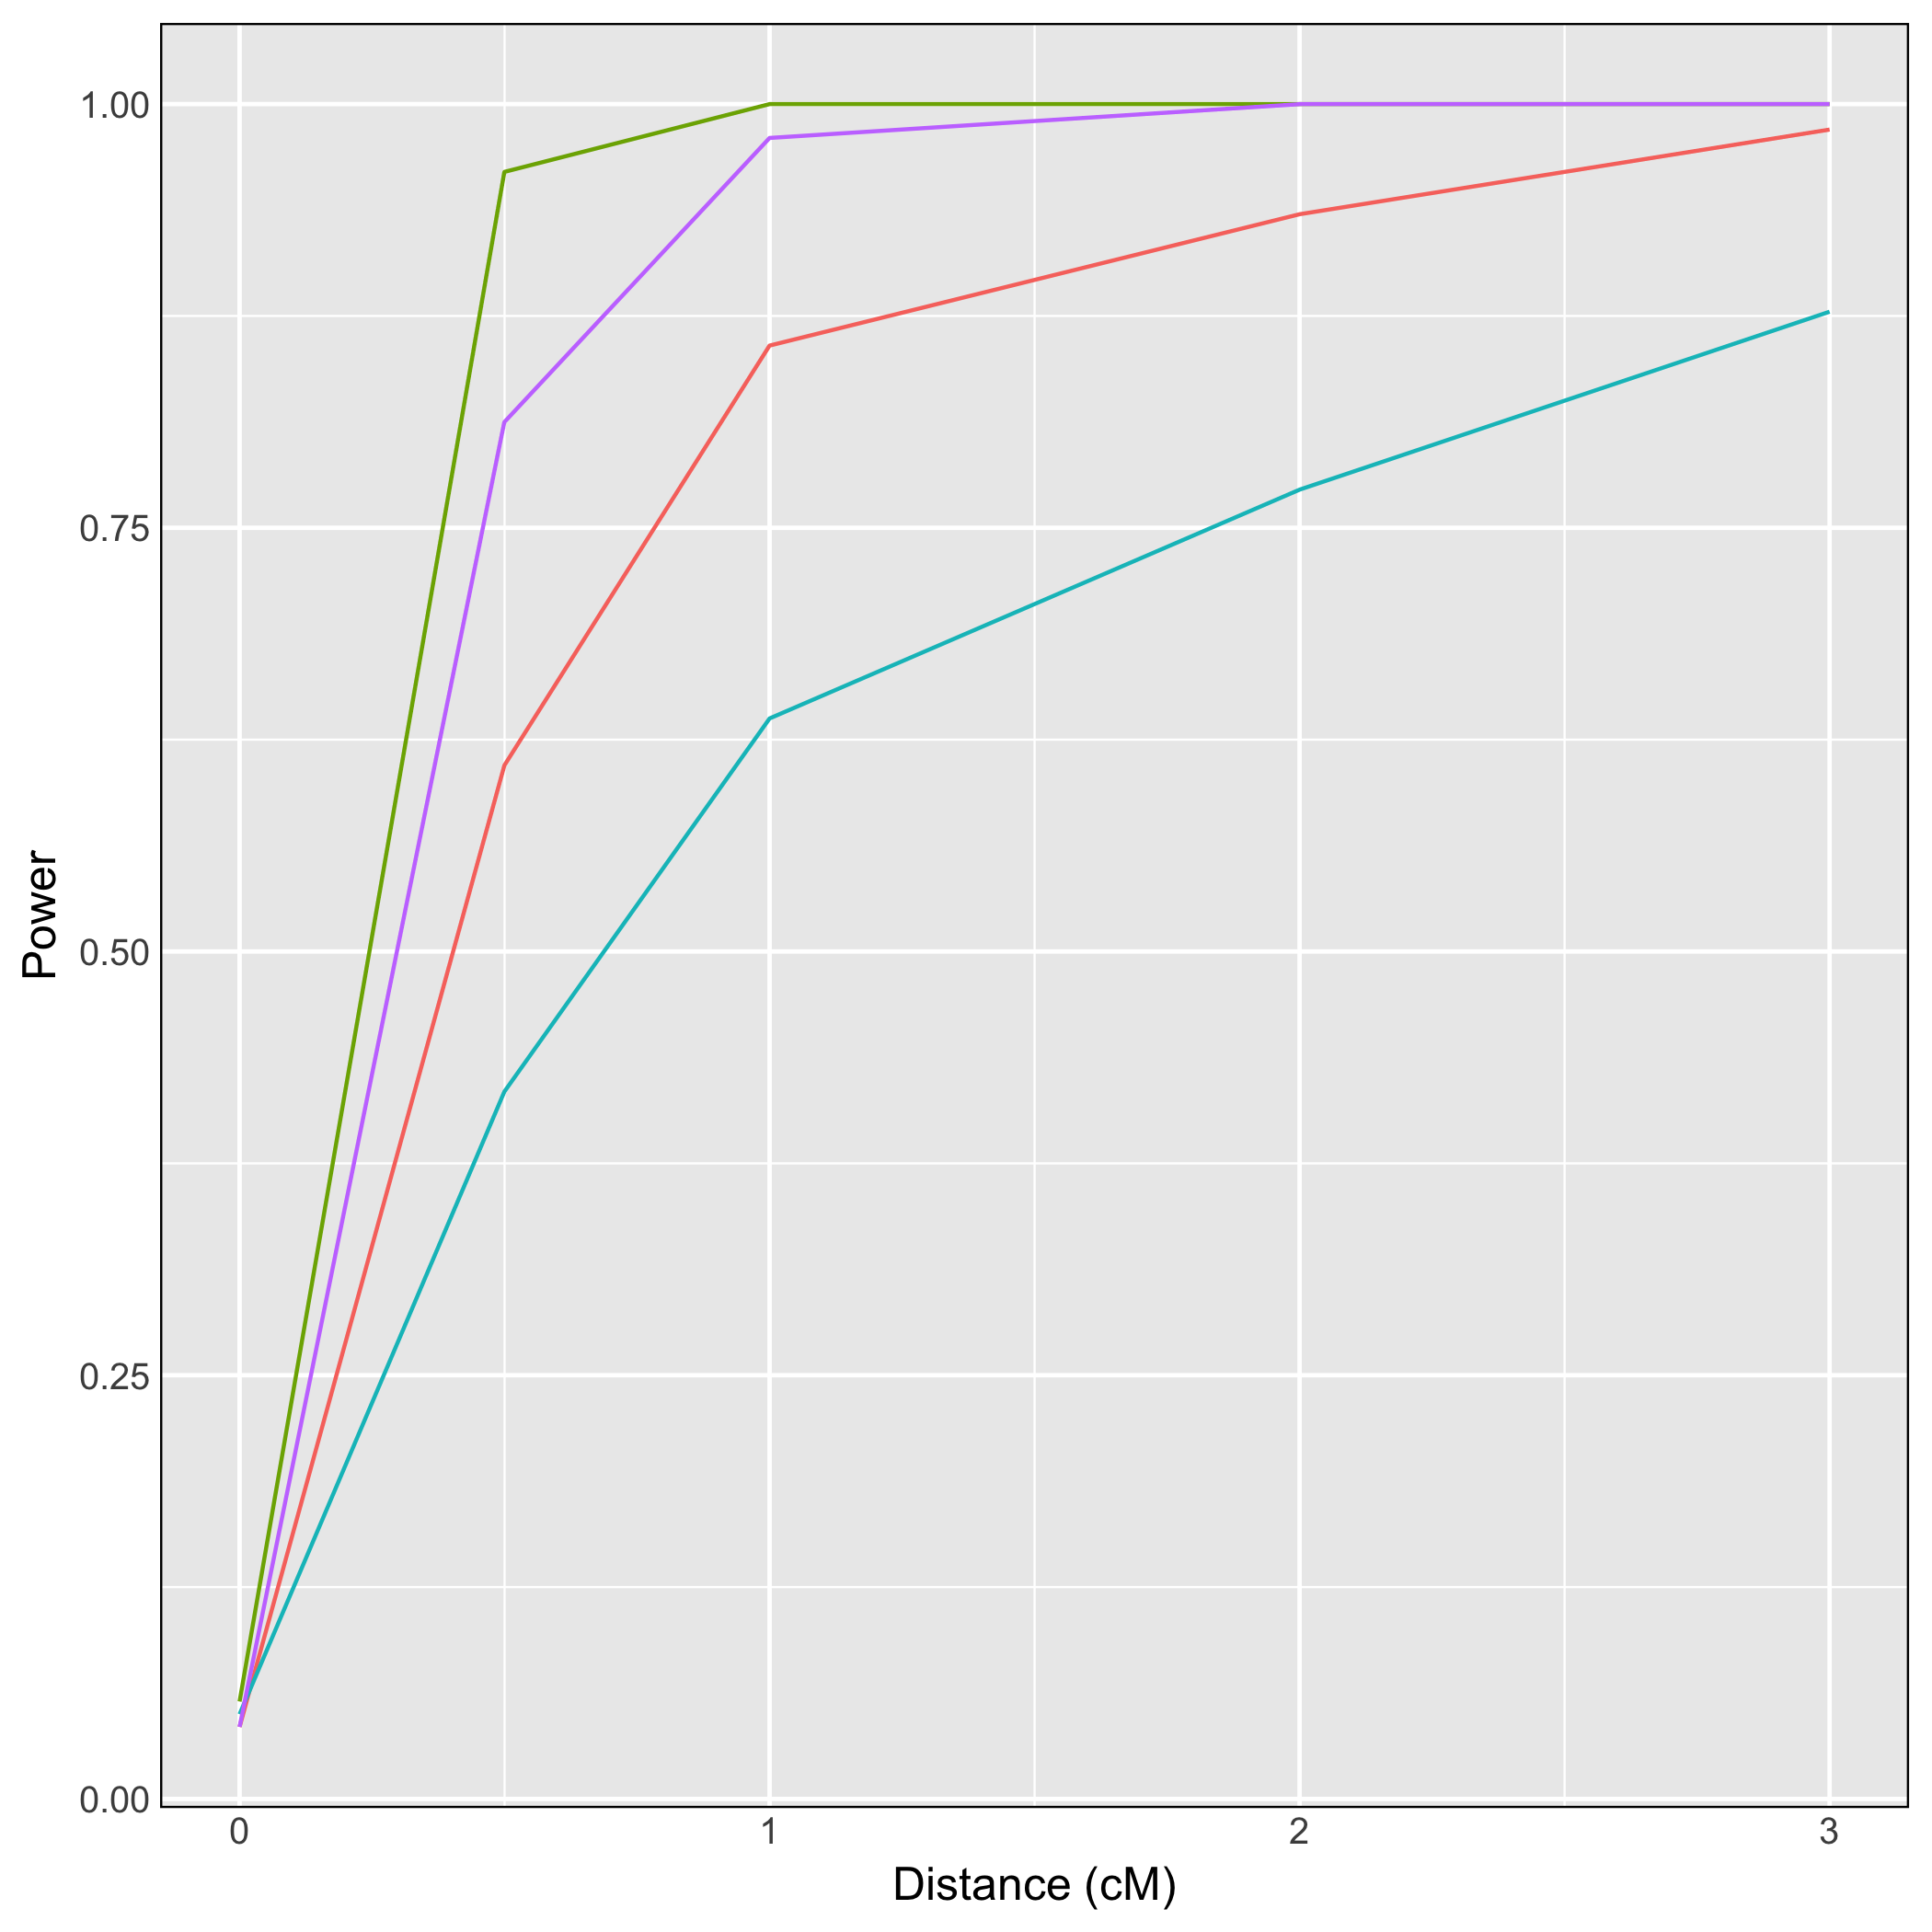
\includegraphics[width = \textwidth]{power-curves}
\caption{Pleiotropy vs. separate QTL power curves for each of four sets of parameter settings. Factors that differ among the four curves are allele effects difference and allele partitioning. Olive green denotes high (2) allele effects difference and allele partitioning into two groups of four. Purple denotes high (2) allele effects difference with unequal allele partitioning. Red and blue both have the low (1) allele effects difference with even and uneven, respectively, allele partitioning.}
\label{fig:power}
\end{figure}

We present our power study results in Figure \ref{fig:power}. Each curve tends upward monotonically as interlocus distance increases. The curve with both the high value, 2, of allele effects difference and even allele partitioning into two groups of four founder alleles uniformly has the greatest power (olive green in Figure \ref{fig:power}). The purple curve denotes the parameter input sets with uneven allele partitioning (F:ABCDEGH) and the high value (2) of allele effects difference. The two curves - red and blue - with the low value, 1, of allele effects difference are uniformly less powerful than those with the high value of allele effects difference. Within the two curves with allele effects difference equal to one, that with the even partitioning (ABCD:EFGH) of founder alleles has uniformly greater power. 


\section{Application}
\label{sec:app}

To illustrate our methods, we applied our test to data from \citet{logan2013high} and \citet{recla2014precise}. \citet{logan2013high} identified two phenotypes - "percent time in light" and "distance traveled in light" - that mapped to 55 cM on chromosome 8. This genomic region intrigued us because \citet{recla2014precise} identified \textit{Hydin} as the gene that underlies the mapping of "hot plate latency" to 57 cM (Supplementary figures). This led us to ask whether \textit{Hydin} affects "percent time in light". We ignored "distance traveled in light" because of its high correlation (Pearson correlation 0.89) with "percent time in light". 




We downloaded and formatted the data from the Mouse Phenome Database \citep{bogue2015collaborative}. We inserted pseudomarkers at 0.1 cM intervals to bring the number of genome-wide markers to 20,183. We used three data structures: one for genotype data, one for phenotype data, and a third for covariates data. For each mouse and each marker, we have eight founder allele probabilities. We structured the allele probabilities for each chromosome as a 261 by 8 by $m_i$ three-dimensional array, where $m_i$ denotes the number of markers on chromosome $i$. We arranged phenotype data into a 261 by 3 matrix, where each column was a single phenotype and each row corresponded to a single mouse. We used only the sex covariate in our analyses. 

We briefly describe the phenotypes that \citet{logan2013high} and \citet{recla2014precise} measured. Both "percent time in light" and "distance traveled in light" were measured by placing mice in a light-dark box, consisting of an insert dividing an open-field apparatus into a light component and a dark component. \citet{logan2013high} then measured the percentage of 20 minutes time spent in the light component of the light-dark box. "Hot plate latency" reflects pain reflexes in response to a thermal stimulus, as recorded by a hot plate analgesia meter. Each mouse remained on the plate until it performed either of two behaviors regarded as indicative of nociception: hindpaw lick or hindpaw shake/flutter.




To determine whether \textit{Hydin} affects "percent time in light", we examined a phenotype scatter plot, performed a test of pleiotropy vs. separate QTL, and created founder allele effects plots. A scatter plot revealed that "percent time in light" and "hot plate latency" are not highly correlated, with a Pearson correlation coefficient of $-0.15$ (Figure \ref{fig:scatter}). 

\begin{figure}
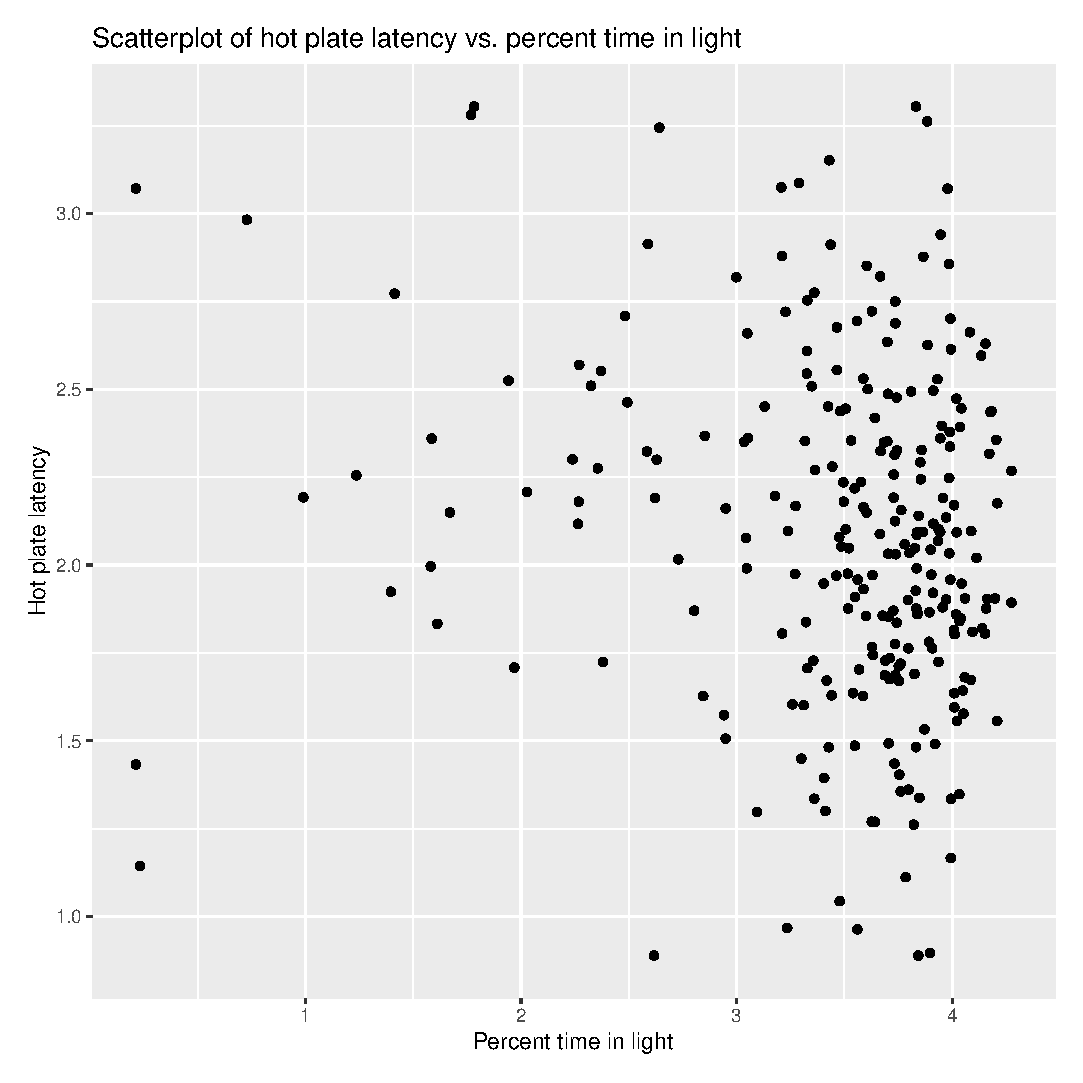
\includegraphics[width = \textwidth]{2018-11-19-scatter.eps}
\caption{Scatter plot of "hot plate latency" against "percent time in light", after applying logarithm transformations and winsorizing both traits.}
\label{fig:scatter}
\end{figure}


\begin{figure}
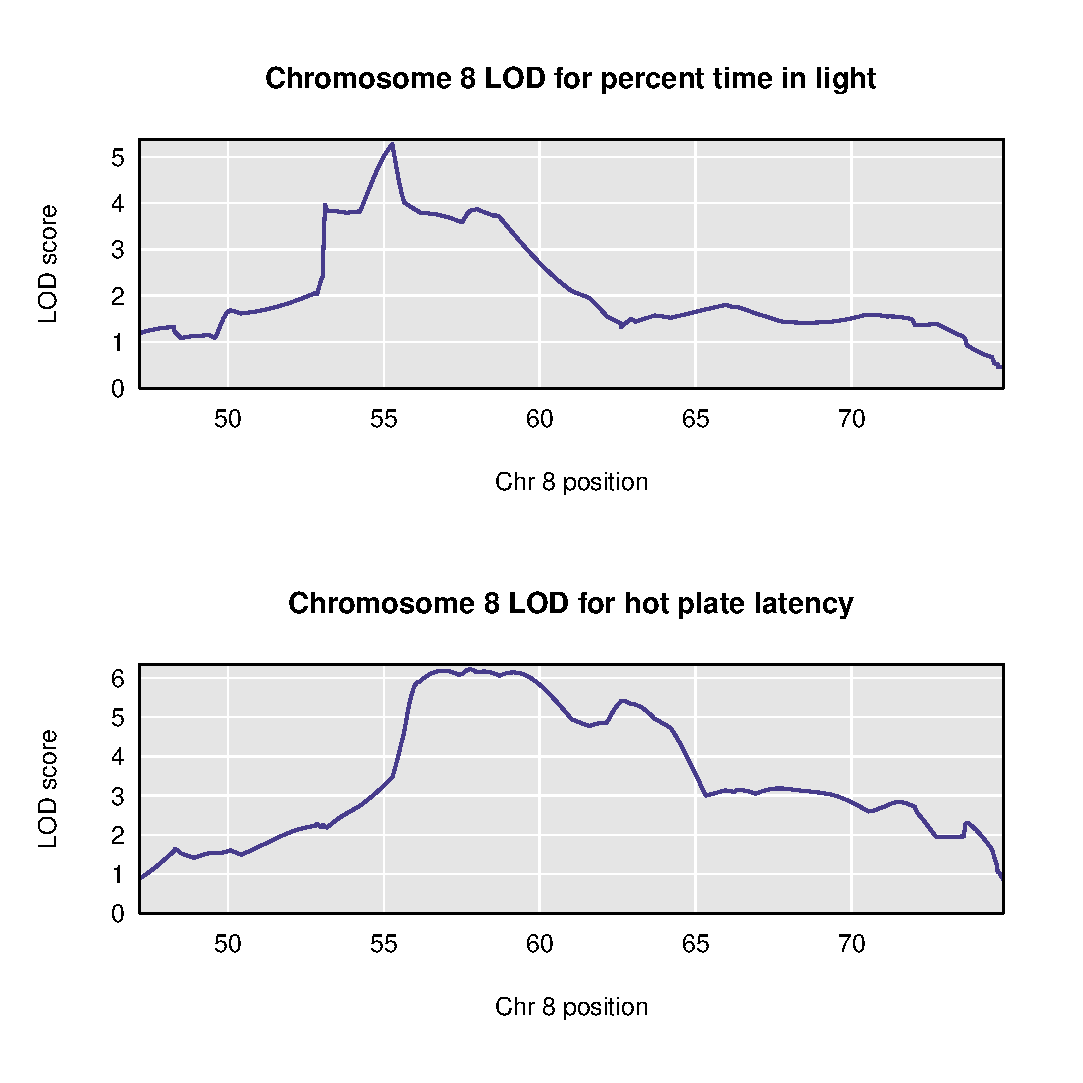
\includegraphics[width = \textwidth]{2018-11-19-chr8-lods.eps}
\caption{Chromosome 8 univariate LOD scores for percent time in light and hot plate latency reveal broad, overlapping peaks between 53 cM and 64 cM. The peak for percent time in light spans the region from approximately 53 cM to 60 cM, with a maximum near 55 cM. The peak for hot plate latency begins near 56 cM and ends about 64 cM.}
\label{fig:chr8-lod}
\end{figure}



In examining the founder allele effects plot for "percent time in light", we see that the purple (WSB) and red (PWK) alleles have high effects near 55 cM, while the navy blue (NOD) has a dramatically lower value (Figure \ref{fig:chr8-effects}). The allele effects plot for "hot plate latency", on the other hand, features a noticeably distinct pattern of allele effects near 55 to 60 cM (Figure \ref{fig:chr8-effects}). Specifically, it has grey (B6) and green (CAST) alleles with much lower effects, while the pink (129), yellow (AJ), purple (WSB), and light blue (NZO) all show higher allele effects in this region.

\begin{figure}
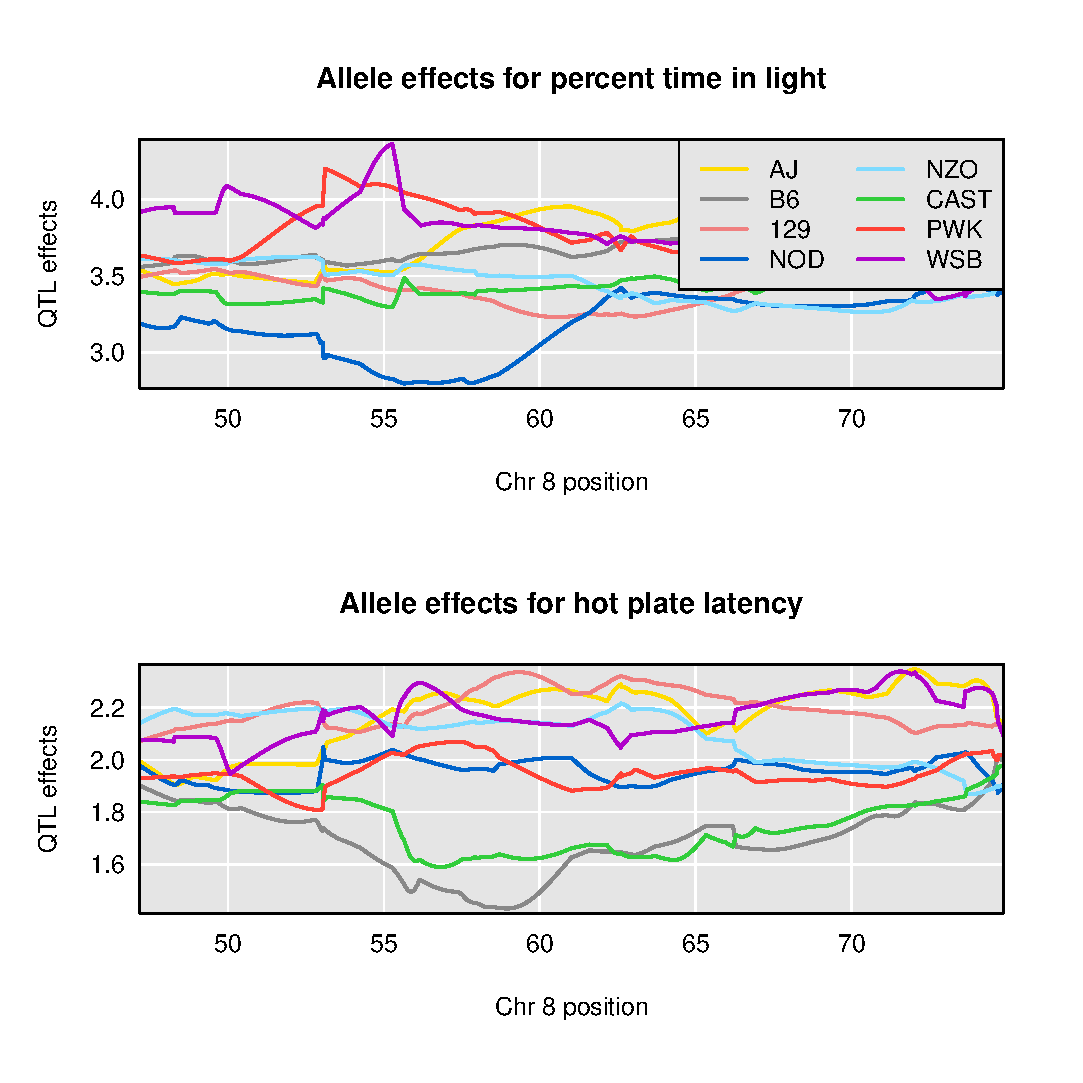
\includegraphics[width = \textwidth]{2018-11-19-coefs.eps}
\caption{Chromosome 8 univariate LOD scores for percent time in light and hot plate latency reveal broad, overlapping peaks between 53 cM and 64 cM. The peak for percent time in light spans the region from approximately 53 cM to 60 cM, with a maximum near 55 cM. The peak for hot plate latency begins near 56 cM and ends about 64 cM.}
\label{fig:chr8-effects}
\end{figure}




We then performed a two-dimensional QTL scan for the pair of phenotypes. With these results, we created a profile LOD plot (Figure \ref{fig:profiles}). The profile LOD plot for the analysis of "percent time in light" and "hot plate latency" displays a peak in the "percent time in light" profile LOD trace near 55 cM; in fact, it overlaps perfectly with the univariate LOD peak for "percent time in light". "Hot plate latency", on the other hand, demonstrates a broad peak in the profile LOD trace, with the maximum achieved near 57 cM (Figure \ref{fig:profiles}A). The pleiotropy trace maximum occurs, too, near 57 cM. The maximal heights of the two profile LOD traces are near 1.2, which is the likelihood ratio test statistic value.

Using the two-dimensional QTL scan results, we calculated a likelihood ratio test statistic value: 1.20. We also calculated a bootstrap p-value with $b = 1000$. The p-value was 0.109. Having set type I error rate $\alpha = 0.05$, this p-values led us to fail to reject the null hypothesis of pleiotropy. 


\begin{figure}
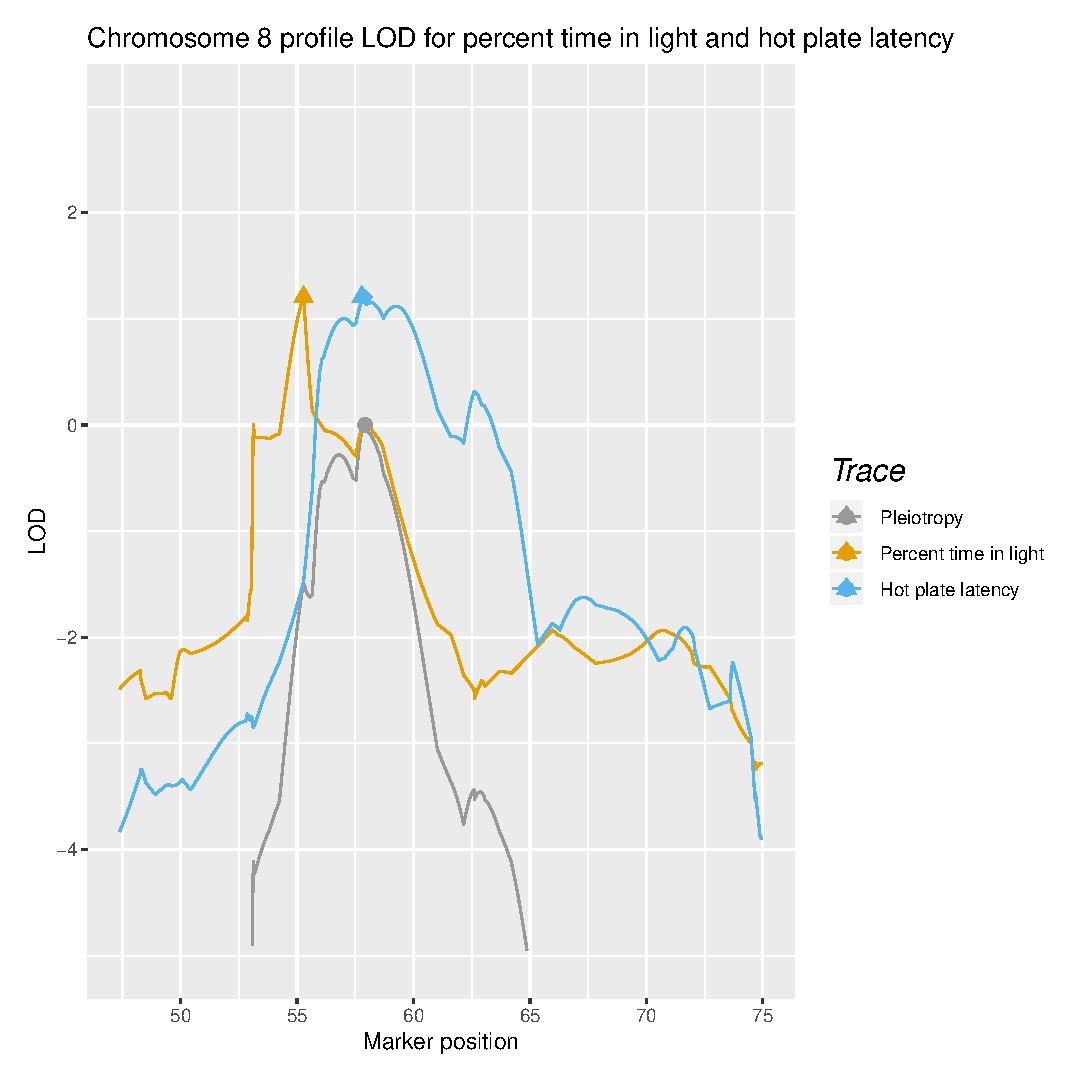
\includegraphics[width = \textwidth]{2018-11-19-profile.eps}
\caption{Profile LOD curves for the pleiotropy vs. separate QTL hypothesis test for "percent time in light" and "hot plate latency". Gray trace denotes pleiotropy LOD values. Triangles denote the univariate LOD maxima, while diamonds denote the profile LOD maxima. For "percent time in light", the yellow triangle obscures the smaller yellow diamond. Likelihood ratio test statistic value corresponds to the height of the blue and yellow traces at their maxima.}
\label{fig:profiles}
\end{figure}







%The results and discussion should not be repetitive. The results section should give a factual presentation of the data and all tables and figures should be referenced; the discussion should not summarize the results but provide an interpretation of the results, and should clearly delineate between the findings of the particular study and the possible impact of those findings in a larger context. Authors are encouraged to cite recent work relevant to their interpretations. Present and discuss results only once, not in both the Results and Discussion sections. It is sometimes acceptable to combine results and discussion. The text should be as succinct as possible. Heed Strunk and White's dictum: "Omit needless words!"

%\section{Additional guidelines}

%\subsection{Numbers} In the text, write out numbers nine or less except as part of a date, a fraction or decimal, a percentage, or a unit of measurement. Use Arabic numbers for those larger than nine, except as the first word of a sentence; however, try to avoid starting a sentence with such a number.

%\subsection{Units} Use abbreviations of the customary units of measurement only when they are preceded by a number: "3 min" but "several minutes". Write "percent" as one word, except when used with a number: "several percent" but "75\%." To indicate temperature in centigrade, use ° (for example, 37°); include a letter after the degree symbol only when some other scale is intended (for example, 45°K).

%\subsection{Nomenclature and Italicization} Italicize names of organisms even when  when the species is not indicated.  Italicize the first three letters of the names of restriction enzyme cleavage sites, as in HindIII. Write the names of strains in roman except when incorporating specific genotypic designations. Italicize genotype names and symbols, including all components of alleles, but not when the name of a gene is the same as the name of an enzyme. Do not use "+" to indicate wild type. Carefully distinguish between genotype (italicized) and phenotype (not italicized) in both the writing and the symbolism.

%\subsection{Cross References}
%Use the \verb|\nameref| command with the \verb|\label| command to insert cross-references to section headings. For example, a \verb|\label| has been defined in the section \nameref{sec:materials:methods}.

%\section{In-text Citations}

%Add citations using the \verb|\citep{}| command, for example  or for multiple citations, 

%\section{Examples of Article Components}
%\label{sec:examples}

%The sections below show examples of different header levels, which you can use in the primary sections of the manuscript (Results, Discussion, etc.) to organize your content.

%\section{First level section header}

%Use this level to group two or more closely related headings in a long article.

%\subsection{Second level section header}

%Second level section text.

%\subsubsection{Third level section header:}

%Third level section text. These headings may be numbered, but only when the numbers must be cited in the text. 

%\section{Figures and Tables}

%Figures and Tables should be labelled and referenced in the standard way using the \verb|\label{}| and \verb|\ref{}| commands.

\section{Discussion}
 
We developed a test of pleiotropy vs. separate QTL for multiparental populations, characterized it with simulation studies, and applied it to answer a scientific question in behavioral genetics. Our simulation studies indicate that the test has power to detect presence of separate loci, especially when univariate trait associations are strong (Figure \ref{fig:power}). Type I error rates indicate that our test is slightly conservative (Table \ref{table-typeI}).

We applied our test to two behavioral phenotypes in a study of 261 Diversity Outbred mice \citep{recla2014precise,logan2013high}. Our results suggest the presence of two distinct QTL, with one QTL (that containing \textit{Hydin}) affecting only "hot plate latency" and a second QTL affecting "percent time in light" (Figure \ref{fig:profiles}). While our p-value of 0.109 led us to fail to reject the pleiotropy hypothesis, the modest p-value suggests the possibility of two distinct loci.

Founder allele effects plots provide further evidence for the presence of two distinct loci. As \citet{macdonald2007joint} and \citet{king2012genetic} argue in their analyses of multiparental *Drosophila* populations, a biallelic pleiotropic QTL would result in allele effects plots that have similar patterns. While we don't know that "percent time in light" and "hot plate latency" arise from biallelic QTL, the dramatic differences that we observe in allele effects patterns further support the argument for two distinct loci, with *Hydin* affecting only "hot plate latency". 


Before discussing future directions for our research, we consider limitations of our current software and methods. Analyses with \texttt{qtl2pleio} are slow. One factor contributing to this is the fact that we wrote \texttt{qtl2pleio} mostly in R. R, due to its design, is slower than many compiled languages, such as C++ \citep{wickham2014advanced}. To accelerate our multi-dimensional QTL scans, we integrated C++ code into \texttt{qtl2pleio} \citep{eddelbuettel2011rcpp}.

Another computational bottleneck is the estimation of variance components $V_g$ and $V_e$. In future research, where we may develop tests for simultaneous analysis of more than two traits, we will consider other strategies for variance component estimation, including that described by \citet{hannah2018limmbo}, who implement a bootstrap strategy to estimate variance components for lower-dimensional phenotypes before combining bootstrap variance component estimates into valid covariance matrices for the full multivariate phenotype. We'll add this variance component estimation method to \texttt{qtl2pleio} by using the \texttt{reticulate} R package to expose objects from the python module \texttt{limmbo} \citep{reticulate}. 


We now contrast pleiotropy vs. separate QTL tests with mediation tests in efforts to illustrate their complementary roles. Many systems genetics investigations apply mediation tests and related methods to infer biomolecular causal relationships \citep{chick2016defining,schadt2005integrative,baron1986moderator}. A mediation test proceeds by including a putative mediator as a covariate in the regression analysis of phenotype and QTL. If a putative mediator sufficiently diminishes the LOD score, then the putative mediator is declared a mediator of the phenotype-QTL relationship.

An important distinction lies in the different goals for mediation tests and pleiotropy vs. separate QTL tests. In a mediation test, we seek to identify mediators of a phenotype-QTL relationship from a collection of putative mediators. In a pleiotropy vs. separate QTL test, one examines two (or more) phenotypes and inquires about the number of distinct QTL. A pleiotropy vs. separate QTL test provides information about the number of underlying QTL, while a mediation test offers conclusions about the relative ordering of biological intermediates within a molecular pathway. 

Despite their distinct goals, \citet{schadt2005integrative} argue that both a pleiotropy vs. separate QTL test and causal inference methods, such as mediation tests, may contribute to gene network reconstruction. They develop a model selection strategy, based on Akaike information criterion \citep{akaike1974new}, to determine which causal model is most compatible with the observed multivariate phenotype data \citep{schadt2005integrative}. In this context, \citet{schadt2005integrative} extend the methods of \citet{jiang1995multiple} to consider more complicated alternative hypotheses, such as the possibility of two QTL, one of which associates with both traits, and one of which associates with only one trait. As envisioned by \citet{schadt2005integrative}, we foresee complementary roles emerging for our pleiotropy vs. separate QTL test and mediation tests in the dissection of complex trait genetic architecture.

Two trends make our scientific contributions especially timely: the accelerating ability of biologists to measure tens of thousands of traits in model organisms and the proliferation of model organism multiparental populations in diverse species. Technological advances in mass spectrometry and RNA sequencing enable the acquisition of high-dimensional biomolecular phenotypes \citep{ozsolak2011rna,han2012multi}. Multiparental populations in \textit{Arabidopsis}, maize, wheat, oil palm, rice, \textit{Drosophila}, yeast, and other organisms enable high-precision QTL mapping \citep{yu2008genetic, tisne2017identification, stanley2017genetic, raghavan2017approaches, mackay2012drosophila, kover2009multiparent, cubillos2013high}. The need to analyze high-dimensional phenotypes in multiparental populations compels the scientific community to develop tools to study genotype-phenotype relationships and complex trait architecture. Our test, and its future extensions, will contribute to these ongoing efforts. 




\subsection*{Acknowledgments}

This research was performed using the compute resources and assistance of the UW-Madison Center For High Throughput Computing (CHTC) in the Department of Computer Sciences. The CHTC is supported by UW-Madison, the Advanced Computing Initiative, the Wisconsin Alumni Research Foundation, the Wisconsin Institutes for Discovery, and the National Science Foundation, and is an active member of the Open Science Grid, which is supported by the National Science Foundation and the U.S. Department of Energy's Office of Science. 

We thank Lindsay Traeger, Julia Kemis, and Rene Welch for critiquing early versions of the manuscript. 

This work was supported in part by National Institutes of Health grant R01GM070683 (to K.W.B.).
\bibliography{research,qtl2pleio-manuscript}

\newpage
\appendix
\section{Supplementary tables}


\begin{center}
\begin{table}
\small
  \begin{tabular}{ c | c }
    \hline
    Founder allele & One-letter abbreviation \\ \hline
    A/J & A \\ 
    C57BL/6J & B \\
    129S1/SvImJ & C \\
    NOD/ShiLtJ & D\\ 
    NZO/H1LTJ & E\\ 
    Cast/EiJ & F\\
    PWK/PhJ & G\\ 
    WSB/EiJ & H\\ 
    \hline
  \end{tabular}
  \caption{Eight founder lines and their one-letter abbreviations.}
  \label{table-letters}
  \end{table}
  
  % latex table generated in R 3.5.1 by xtable 1.8-3 package
% Tue Nov 20 10:28:47 2018
\begin{table}[ht]
\begin{tabular}{l|lrr}
  \hline
lodcolumn & chr & pos & lod \\ 
   \hline
percent time in light & 8 & 55.28 & 5.27 \\ 
 hot plate latency & 8 & 57.77 & 6.22 \\ 
 percent time in light & 9 & 36.70 & 5.42 \\ 
 hot plate latency & 9 & 46.85 & 5.22 \\ 
 percent time in light & 11 & 63.39 & 6.46 \\ 
 hot plate latency & 12 & 43.52 & 5.13 \\ 
 percent time in light & 15 & 15.24 & 5.67 \\ 
 hot plate latency & 19 & 47.80 & 5.48 \\ 
   \hline
\end{tabular}
  \caption{Both "hot plate latency" and "percent time in light" demonstrate multiple QTL peaks with LOD scores above 5.}
  \label{table-peaks}
\end{table}
  
  
  
\end{center}







\newpage
\section{Supplementary figures}
\begin{figure}
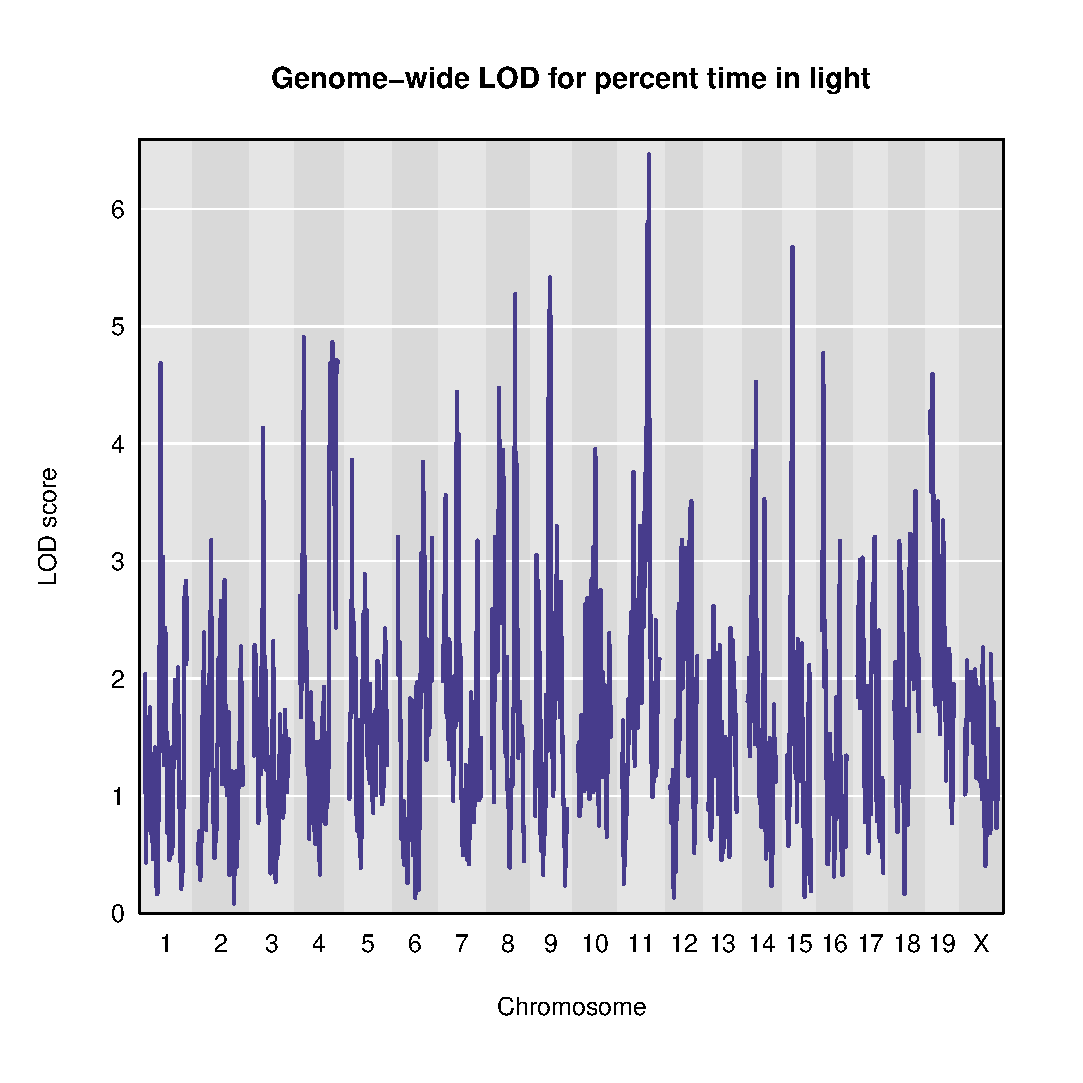
\includegraphics{2018-11-19-genomewide_lod_trait10.eps}
\caption{Genome-wide QTL scan for percent time in light reveals multiple QTL, including one on Chromosome 8.}
\label{fig:genomewide10}
\end{figure}

\begin{figure}
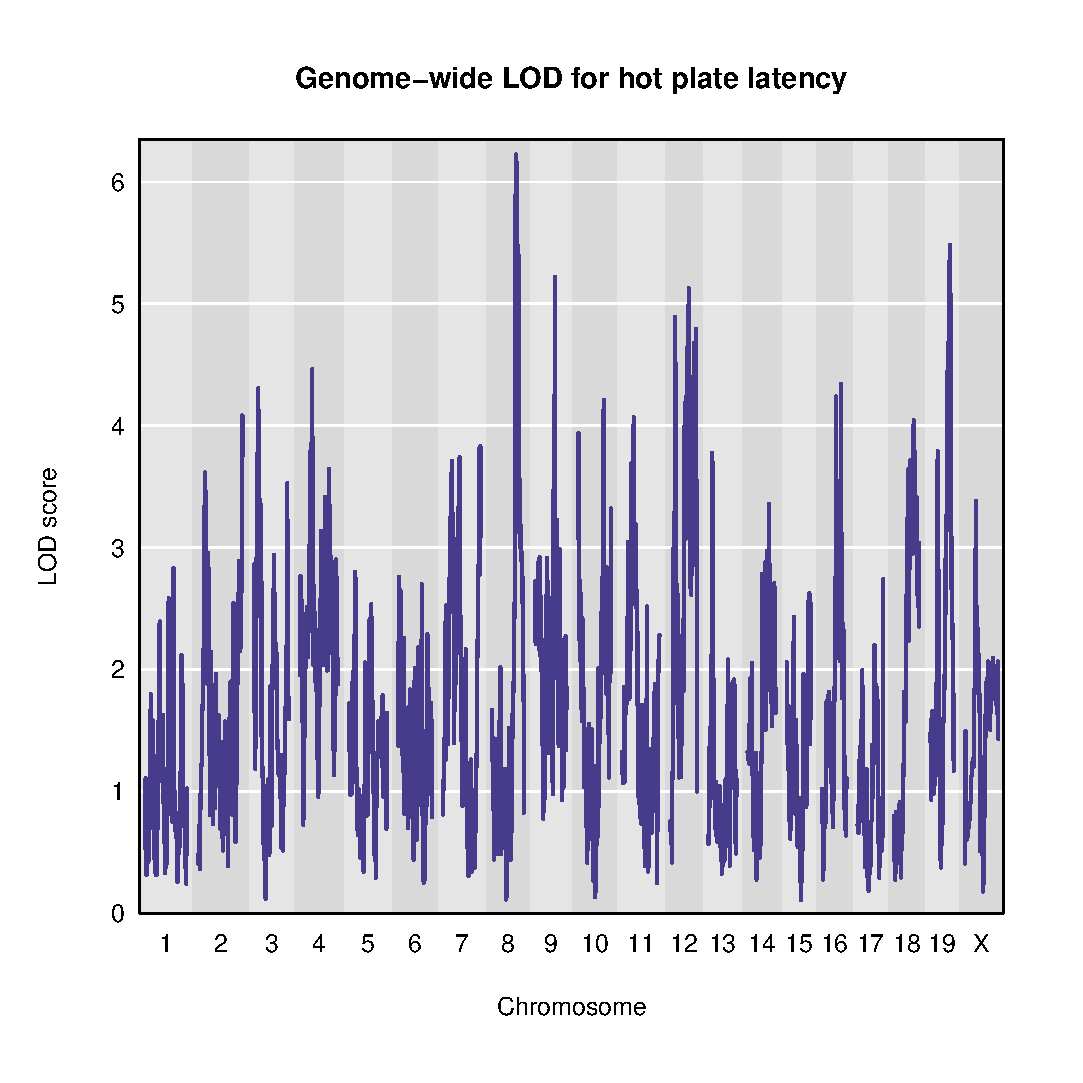
\includegraphics{2018-11-19-genomewide_lod_trait22.eps}
\caption{Genome-wide QTL scan for hot plate latency reveals multiple QTL, including a peak on Chromosome 8.}
\label{fig:genomewide22}
\end{figure}







\end{document}